\documentclass[11pt]{article}

\usepackage[a4paper,margin=0.8in]{geometry}
\usepackage{amsmath,amssymb}
\usepackage{booktabs,longtable,array}
\usepackage{caption}
\usepackage{graphicx}
\usepackage{hyperref}

\newcommand{\code}[1]{\texttt{#1}}
\newcommand{\NA}{--}
\newcommand{\Exp}{\mathrm{Exp}}

\title{Numerical Setup and Interpretation for the Three Hawkes Experiments}
\author{}
\date{}

\begin{document}
\maketitle

This file records the numerical design parameters used in the three experiments
in this archive. The values and
reported costs were audited against the active experiment notebooks and their
current result files on August 11, 2026:
\code{single\_exponential\_check\_experiment/current\_readout\_markov\_ct\_ddpg.ipynb},
\code{complex\_erlang\_experiment/erlang\_kernel\_comparison.ipynb}, and
\code{powerlaw\_kernel\_experiment/powerlaw\_kernel\_comparison.ipynb}.
All three notebooks were executed without cell errors before the accompanying
figure collection was refreshed. All controls are scalar and constrained to
\(a\in[0,1]\). The static benchmark is selected independently in each
environment and then frozen before the common-test evaluation: \(a=0.39\) for
the single-exponential model, \(a=0.26\) for Erlang, and \(a=0.34\) for the
power-law model.

\section{Numerical Setup}

The simulator reports discounted reward internally, whereas the tables and
figures below report the equivalent positive discounted cost. Thus, lower
values indicate better policies. All Monte Carlo comparisons use common test
seeds within an experiment.

\begin{table}[h!]
\centering
\caption{High-level experiment definitions.}
\label{tab:experiment_definitions}
\small
\begin{tabular}{p{0.18\linewidth}p{0.25\linewidth}p{0.25\linewidth}p{0.25\linewidth}}
\toprule
Item & Single exponential & Erlang kernel & Power-law kernel \\
\midrule
Folder &
\code{single\_exponential\_check\_experiment} &
\code{complex\_erlang\_experiment} &
\code{powerlaw\_kernel\_experiment} \\
True kernel &
\(\phi(u)=e^{-1.30u}\) &
\(\phi(u)=\rho u e^{-\rho u}\), \(\rho=1.15\) (the scale is carried by \(\alpha\)) &
\(\phi(u)=b\eta^b(u+\eta)^{-(1+b)}\), \(\eta=0.12,\ b=0.80\) \\
True Markovization &
Exact, one exponential memory is included in the filter bank &
Exact, two Erlang auxiliary states \(Y^1,Y^2\) &
No finite exact Markovization; simulator uses event-history power-law memory \\
CT-DDPG memory state &
Exponential filter bank \(Z^k\), \(K=8\) &
Exponential filter bank \(Z^k\), \(K=12\) &
Exponential filter bank \(Z^k\), \(K=20\) \\
DGM/HJB oracle &
Known-parameter exact single-exponential Markov state &
Known-parameter exact Erlang Markov state &
Known-parameter exponential-mixture approximation with positive memory link \\
Generic RL baselines &
Not used in this sanity-check experiment &
SAC and DDPG with current-state and filtered observations &
SAC and DDPG with current-state and filtered observations \\
\bottomrule
\end{tabular}
\end{table}

\begin{longtable}{p{0.23\linewidth}p{0.23\linewidth}p{0.23\linewidth}p{0.23\linewidth}}
\caption{Environment and objective parameters.}
\label{tab:environment_parameters}\\
\toprule
Parameter & Single exponential & Erlang kernel & Power-law kernel \\
\midrule
\endfirsthead
\toprule
Parameter & Single exponential & Erlang kernel & Power-law kernel \\
\midrule
\endhead
\bottomrule
\endfoot
Horizon \(T\) & \(5.0\) & \(5.0\) & \(8.0\) \\
Time step \(\Delta t\) & \(0.02\) & \(0.02\) & \(0.02\) \\
Discount rate \(\beta_{\rm disc}\) & \(0.02\) & \(0.02\) & \(0.02\) \\
Baseline \(\mu(t,x,a)\) &
\(\operatorname{clip}(2.05+0.10x-0.08a,10^{-6},6)\) &
\(\operatorname{clip}(2.00+0.03x-0.04a,10^{-6},5)\) &
\(\operatorname{clip}(0.60+0.002x-0.002a,10^{-6},5)\) \\
Excitation scale \(\alpha\) & \(1.25\) & \(1.05\) & \(0.99\) \\
Control effectiveness \(q(a)\) &
\(c_a=1.25,\ a_{1/2}=0.35\) &
\(c_a=1.30,\ a_{1/2}=0.35\) &
\(c_a=1.08,\ a_{1/2}=0.10\), where \(q(a)=1-c_a a/(a_{1/2}+a)\) \\
Total intensity cap & None & None & None \\
Filter decays &
\(0.325k,\ k=1,\ldots,8\); true decay \(1.30\) is filter \(k=4\) &
\(0.23k,\ k=1,\ldots,12\); Erlang decay \(1.15\) is filter \(k=5\) &
\(1.00k,\ k=1,\ldots,20\) \\
Mixture weights &
Exact single-exponential readout &
Exact Erlang oracle; signed diagnostic fit for filters &
Signed ridge fit from exponential mixture; positive part applied to approximated memory readout \\
Drift \(b(x,a)\) &
\(0.02-0.45x-0.72a\) &
\(0.02-0.45x-0.70a\) &
\(-1.00x-0.02a\) \\
Volatility \(\sigma(x,a)\) &
\([0.05+0.015x+0.08a]_+\) &
\([0.05+0.012x+0.08a]_+\) &
\([0.03+0.002x+0.005a]_+\) \\
Jump amplitude \(\gamma(x,a)\) &
\(\operatorname{clip}(0.10+0.015x-0.015a,10^{-4},0.25)\) &
\(\operatorname{clip}(0.085+0.005x-0.010a,10^{-4},0.20)\) &
\(\operatorname{clip}(0.50+0.002x-0.05a,10^{-4},0.90)\) \\
State running-cost coefficient \(c_x\) & \(0.80\) & \(0.3000\) & \(1.00\) \\
Control running-cost coefficient \(c_a^{\rm cost}\) & \(0.18\) & \(0.2250\) & \(0.50\) \\
Event-count running-cost coefficient \(c_N\) & \(0\) & \(0\) & \(0\) \\
Terminal-cost coefficient \(c_T\) & \(0.60\) & \(0.2250\) & \(0.50\) \\
Worst-case finite-horizon offspring mass & \(0.96009\) & \(0.89343\) & \(0.95601\) \\
Approximation-envelope mass & \(0.96009\) & \(0.89343\) & \(0.93837\) \\
\end{longtable}

There is no clipping of the \emph{total} intensity in any experiment. The
baseline and jump-amplitude clips in Table~\ref{tab:environment_parameters}
are bounded coefficient specifications, not intensity caps. Event arrivals
therefore remain fully endogenous, and the running objective is
\[
  \ell(x,a)=c_xx^2+c_a^{\rm cost}a^2,
  \qquad g(x)=c_Tx^2,
\]
with no separate event-count penalty.

For a transparent sufficient-condition check, let
\(\bar q=\sup_{a\in[0,1]}q(a)=1\). On \([0,T]\), the true excitation masses are
\[
\begin{aligned}
M_{\rm exp}
 &=1.25\int_0^5 e^{-1.30u}\,du=0.96009,\\
M_{\rm Erlang}
 &=1.05\int_0^5 1.15u e^{-1.15u}\,du=0.89343,\\
M_{\rm power}
 &=0.99\int_0^8 0.80(0.12)^{0.80}(u+0.12)^{-1.80}\,du=0.95601.
\end{aligned}
\]
All are strictly below one. The signed exponential approximations are checked
through their positive-link envelope, whose corresponding masses are also
below one as reported in the table. Together with compact controls, bounded
baseline and jump coefficients, finite horizon, and the displayed Lipschitz
coefficients, this gives the subcritical sufficient route used to verify the
moment requirement in Assumption~3.2 (with the numerical diagnostic using
\(p_*=4\)). Since the quadratic costs have growth index \(q=1\), this also
gives \(p_*>q+1=2\). The uncapped Monte Carlo plots included in each notebook are
stress checks for the calibration; they are not substituted for this
analytical certificate.

\begin{longtable}{p{0.26\linewidth}p{0.20\linewidth}p{0.20\linewidth}p{0.20\linewidth}}
\caption{CT-DDPG training parameters.}
\label{tab:ctddpg_parameters}\\
\toprule
Parameter & Single exponential & Erlang kernel & Power-law kernel \\
\midrule
\endfirsthead
\toprule
Parameter & Single exponential & Erlang kernel & Power-law kernel \\
\midrule
\endhead
\bottomrule
\endfoot
Maximum training episodes & \(220\) & \(140\) & \(180\) \\
Warmup episodes & \(25\) & \(30\) & \(30\) \\
Updates per episode & \(10\) & \(10\) & \(10\) \\
Validation frequency & every \(20\) episodes & every \(20\) episodes & every \(20\) episodes \\
Validation episodes during training & \(160\) & \(100\) & \(120\) \\
Validation early stopping & restore best checkpoint & five evaluations without improvement & six evaluations without improvement \\
Network hidden sizes & \((48,48)\) & \((64,64)\) & \((64,64)\) \\
Replay segment length & \(50\) & \(64\) & \(64\) \\
Critic batch size & \(128\) & \(192\) & \(192\) \\
Actor batch size & \(256\) & \(384\) & \(384\) \\
Actor learning rate & \(2\times10^{-5}\) & \(5\times10^{-6}\) filtered, \(2\times10^{-5}\) current & \(5\times10^{-7}\) filtered, \(5\times10^{-6}\) current \\
Filter-profile learning rate & \(0\) & \(10^{-4}\) filtered, \(0\) current & \(0\) \\
Critic learning rate & \(8\times10^{-4}\) & \(6\times10^{-4}\) & \(6\times10^{-4}\) \\
Polyak parameter \(\tau\) & \(0.01\) & \(0.003\) & \(0.003\) \\
Terminal penalty & \(5.0\) & \(7.5\) & \(7.5\) \\
Gradient clip & \(10.0\) & \(5.0\) & \(5.0\) \\
Replay capacity & \(500\) episodes & \(180\) episodes & \(180\) episodes \\
Initial actor level & \(0.30\) & \(0.16\) filtered, \(0.22\) current & \(0.18\) for both modes \\
Actor skip coefficients &
\(x:6.0,\ z:0.5\) &
\(t:0,\ x:6.00,\ \sum_k z_k:1.00\) filtered; \(x:1.20\) current &
filtered warm start inherits \(x:2.00\), with filter level \(2.00\), rate slope \(2.00\), and logit shift \(-0.30\); \(x:2.00\) current \\
Actor-update frequency & every critic update & every critic update & every second critic update filtered; every critic update current \\
Target networks &
Target value only in this diagnostic implementation &
Target actor and target value &
Target actor and target value \\
\end{longtable}

\begin{longtable}{p{0.26\linewidth}p{0.20\linewidth}p{0.20\linewidth}p{0.20\linewidth}}
\caption{Oracle, generic RL baseline, and evaluation parameters.}
\label{tab:benchmark_parameters}\\
\toprule
Parameter & Single exponential & Erlang kernel & Power-law kernel \\
\midrule
\endfirsthead
\toprule
Parameter & Single exponential & Erlang kernel & Power-law kernel \\
\midrule
\endhead
\bottomrule
\endfoot
DGM steps & \(450\) & \(650\) & \(1200\) \\
DGM batch size & \(256\) & \(384\) & \(512\) \\
DGM hidden dimension & \(64\) & \(72\) & \(96\) \\
DGM layers & \(3\) & \(3\) & \(3\) \\
DGM learning rate & \(2\times10^{-3}\) & \(1.5\times10^{-3}\) & \(1.5\times10^{-3}\) \\
DGM action grid size & \(41\) & \(41\) & \(41\) \\
DGM sampling &
Uniform PDE domain &
Uniform PDE domain &
Reachable-state sampling, \(120\) episodes, \(12\%\) uniform mix \\
DGM validation/restoration &
\NA &
\NA &
Validate every \(150\) steps using \(64\) episodes; restore best checkpoint \\
SAC/DDPG training &
Not run &
SAC current \(180{,}000\), SAC filtered \(220{,}000\), DDPG \(160{,}000\) maximum transitions &
SAC current \(100{,}000\), SAC filtered \(200{,}000\), DDPG current \(120{,}000\), DDPG filtered \(160{,}000\) maximum transitions \\
SB3 observation modes &
\NA &
\code{current} and \code{filters} &
\code{current} and \code{filters} \\
SB3 feature conditioning &
\NA &
Current: \((t,X)\); filters: all 12 normalized observed levels; SAC also uses 11 adjacent decay-rate differences computed from the same bank &
Current: \((t,X)\); filters: all 20 normalized observed filter levels \\
SB3 vectorized environments &
\NA &
\(4\) for SAC and DDPG &
\(4\) for SAC and DDPG \\
SB3 learning rate and batch size &
\NA &
SAC and DDPG \(1\times10^{-4}\); batch \(512\) &
SAC current \(2\times10^{-4}\), SAC filtered \(10^{-4}\), batch \(512\); both DDPG variants \(5\times10^{-5}\), batch \(1024\) \\
SAC/DDPG replay updates &
\NA &
\(1\) update per four-environment vector step &
SAC filtered: \(2\) updates per four-environment vector step; all others: \(1\) \\
SB3 discount during training &
\NA &
\(\exp(-0.02\cdot0.02)\approx0.999600\) &
\(\exp(-0.02\cdot0.02)\approx0.999600\) \\
SB3 reward scale &
\NA &
\(25.0\) &
SAC: \(25.0\); DDPG: \(10.0\) \\
DDPG exploration noise &
\NA &
\(0.05\) on internal \([-1,1]\) scale &
\(0.05\) for current and \(0.03\) for filters on internal \([-1,1]\) scale \\
SB3 learning starts &
\NA &
\(5000\) &
SAC: \(5000\); DDPG: \(15{,}000\) \\
DDPG initialization/stabilization &
\NA &
Default actor initialization; optimizer weight decay \(10^{-4}\) &
Current actor initialized at physical action \(0.30\); filtered actor warm-started with zero memory weights; optimizer weight decay \(10^{-4}\) \\
SB3 checkpoint selection &
\NA &
Validate every \(10{,}000\)--\(20{,}000\) transitions using \(64\)--\(96\) common-random episodes; restore the best checkpoint; warm-start filtered SAC/DDPG from current-state checkpoints; selected SAC runs use the full budget &
Validate every \(10{,}000\)--\(12{,}500\) transitions using \(64\)--\(128\) common-random episodes; restore the best checkpoint; warm-start filtered SAC/DDPG from current-state checkpoints; filtered continuations use their full budgets \\
SB3 devices &
\NA &
Four bounded CPU workers for SB3, two for NumPy CT-DDPG; CUDA for DGM &
Four bounded CPU workers for SB3, two for NumPy CT-DDPG; CUDA for DGM \\
Monte Carlo validation episodes &
\(300\) &
\(400\) &
\(800\) \\
Path-ensemble episodes for figures &
\(20\) &
\(20\) &
\(20\) \\
Static benchmark &
\(a\equiv0.39\) &
\(a\equiv0.26\) &
\(a\equiv0.34\) \\
Static-selection validation grid &
\(\{0.36,0.37,\ldots,0.42\}\) &
\(\{0.22,0.23,\ldots,0.28\}\) &
\(\{0.32,0.33,0.34\}\) \\
Static-selection episodes &
\(1{,}200\) &
\(1{,}200\) &
\(1{,}600\) \\
Static-selection seed &
\multicolumn{3}{c}{(1731)} \\
\end{longtable}

\section{Numerical Results}

\begin{table}[h!]
\centering
\caption{Mean discounted cost with 90\% Monte Carlo intervals. Lower is better.
The intervals measure rollout uncertainty conditional on one trained policy;
bold values identify the best model-free learned policy in each comparison.}
\label{tab:numerical_results}
\small
\begin{tabular}{p{0.25\linewidth}ccc}
\toprule
Policy & Single exponential & Erlang kernel & Power-law kernel \\
\midrule
DGM/HJB oracle
& \(0.1658\pm0.0070\)
& \(0.1037\pm0.0046\)
& \(1.5696\pm0.0617\) \\
CT-DDPG current
& \NA
& \(0.1219\pm0.0067\)
& \(1.6647\pm0.0634\) \\
CT-DDPG filtered
& \(\mathbf{0.1744}\pm0.0073\)
& \(\mathbf{0.1056}\pm0.0049\)
& \(\mathbf{1.5870}\pm0.0607\) \\
SAC current
& \NA
& \(0.1093\pm0.0050\)
& \(1.7920\pm0.0665\) \\
SAC filtered
& \NA
& \(0.1065\pm0.0046\)
& \(1.7056\pm0.0641\) \\
DDPG current
& \NA
& \(0.1266\pm0.0051\)
& \(1.7669\pm0.0644\) \\
DDPG filtered
& \NA
& \(0.1103\pm0.0050\)
& \(1.7410\pm0.0680\) \\
Validation-selected static
& \(0.3247\pm0.0214\)
& \(0.1314\pm0.0060\)
& \(1.9242\pm0.0734\) \\
\bottomrule
\end{tabular}
\end{table}

In the single-exponential column, \emph{CT-DDPG filtered} denotes the proposed
CT-DDPG supplied with the eight-filter bank. Because the fourth decay equals
the true decay, this bank contains an exact Markov representation. SAC and
standard DDPG are not included in this sanity-check experiment.

\section{Interpretation}

\paragraph{Single-exponential sanity check.}
The true exponential kernel is represented exactly by one member of the
preselected filter dictionary. CT-DDPG attains cost \(0.1744\), reducing cost
by \(46.3\%\) relative to the independently selected static benchmark
\(a\equiv0.39\), whose cost is \(0.3247\). The known-parameter DGM/HJB oracle
remains better at \(0.1658\), as expected. This experiment
therefore checks that the observed-filter implementation can exploit an exact
finite-dimensional memory state; it is not a comparison against SAC or
standard DDPG, and it does not contain a current-state ablation.

\paragraph{Erlang kernel.}
The oracle uses the exact two-phase Markov state \((X,Y^1,Y^2)\), while all
model-free filtered policies receive only the generic 12-dimensional
exponential filter bank. Relative to current-state observations, filtering
reduces mean cost by \(13.4\%\) for CT-DDPG, \(2.55\%\) for SAC, and \(12.9\%\)
for DDPG. SAC augments the observed levels with generic adjacent-rate finite
differences; it receives no exact Erlang phase or fitted kernel coefficient.
Filtered CT-DDPG is numerically the best learned policy, improving on filtered
SAC and filtered DDPG by \(0.89\%\) and \(4.31\%\), respectively. The exact
DGM/HJB oracle remains the best overall policy, with cost \(0.1037\).

\paragraph{Power-law kernel.}
The true simulator retains the full event history, because the power-law kernel
has no exact finite-dimensional Markov representation. The learning methods
instead observe a 20-dimensional exponential filter approximation, and the
DGM/HJB benchmark solves the corresponding known-parameter mixture problem
before its policy is evaluated in the true-history simulator. The revised
uncapped calibration uses a sharp power-law scale \(\eta=0.12\), branching mass
\(0.99\), and the resolved arithmetic dictionary \((1,2,\ldots,20)\). It uses
zero prehistory, positive unmarked jumps, and no event-count cost. On two
independent 800-path evaluations, filtering reduces CT-DDPG cost by \(4.67\%\)
and \(3.63\%\), respectively. On the seed-999 evaluation reported in the
table, filtered CT-DDPG also improves by \(17.8\%\) over static control. It is
the best model-free learned policy, improving on filtered SAC and filtered
DDPG by \(6.96\%\) and \(8.85\%\), respectively. Filtered SAC improves by
\(4.82\%\) over its current-state ablation, while filtered DDPG improves by
\(1.47\%\). The DDPG direction is repeated on two additional 800-path blocks
after stabilizing its critic-target scale and initialization. The privileged
DGM/HJB oracle remains slightly better at \(1.5696\). The filtered CT-DDPG mean
action is lower while its temporal
variation is higher, consistent with selective intervention during endogenous
clusters.

\paragraph{Cross-experiment conclusion.}
In both maintained memory comparisons, filtered CT-DDPG improves on its
current-state ablation. The Erlang reduction is \(13.4\%\), while the revised
power-law reduction is approximately \(3.6\%\)--\(4.7\%\) across two final
seeds. The single-exponential experiment complements this evidence by showing
that the same filter construction works when its dictionary contains the exact
Markov state. In both non-exponential experiments, filtered CT-DDPG is the best
model-free learned policy and the known-parameter DGM/HJB oracle remains the
best overall reference. Filtered SAC also improves on its current-state
ablation in both experiments; this direction persists on three independent
800-path seed blocks for each kernel.

All methods within a filtered comparison receive the same underlying bank of
observed readouts. The complete CT-DDPG/SAC/DDPG training budgets are
\(35{,}000/220{,}000/160{,}000\) environment transitions for Erlang and
\(72{,}000/200{,}000/160{,}000\) for power law. Thus CT-DDPG's numerical case
rests not only on the lowest model-free mean cost, but also on reaching that
policy with the smallest sample budget. We retain the fully tuned SAC and DDPG
baselines rather than shortening their training to amplify the displayed gap.

These findings support a claim of \emph{directionally consistent numerical improvement}, but
not yet formal statistical superiority. The reported confidence intervals
condition on one trained checkpoint per method and overlap for several
filtered-policy comparisons. A final statistical claim should aggregate
multiple independent training seeds and report uncertainty for paired cost
differences on the common test paths.

\section{Implementation and Reporting Notes}

The single-exponential experiment is mainly a sanity check: the true kernel is
exactly represented by one filter in the CT-DDPG memory bank. The Erlang
experiment has an exact finite Markovian oracle, while CT-DDPG uses the
model-free exponential filter bank. The power-law experiment evaluates CT-DDPG
on the true event-history simulator and uses an exponential-mixture HJB/PINN
oracle as an approximation benchmark. No experiment includes an event-count
cost or a total-intensity cap. Bounded state-jump amplitudes and subcritical
excitation keep the uncapped calibration numerically stable while Hawkes memory
remains decision-relevant. In all finite approximations with signed
kernel coefficients, the positive part is applied only to the approximated
memory readout, not to the full classical Hawkes intensity.
For the generic RL baselines, the network action lies in \([-1,1]\) and is
affinely mapped to the physical control \([0,1]\). Raw filter channels use the
matched scaling \(Z_t^k/z_{\rm scale}\); Erlang SAC instead applies logarithmic
level conditioning and adjacent-rate finite differences. Both preprocessing
maps use only the preselected filter rates and observed filter states. In the Erlang
experiment, the base filtered observation contains \((t,X)\) and all 12
normalized filter levels, giving dimension 14, compared with 2 for the
current-state observation. Erlang SAC augments these levels with 11 adjacent
decay-rate differences, giving input dimension 25 but no additional stochastic
information. The corresponding power-law dimensions are 22 and 2. Filtered
SAC and DDPG use tuned learning rates and Polyak parameters; power-law
filtered policies are warm-started from their respective current-state
checkpoints in both memory experiments. The Erlang filtered actor additionally learns a zero-initialized
three-coefficient residual over filter level, decay-rate slope, and curvature.
This residual uses only the observed filter bank and the preselected decay
grid; it is updated by the CT-DDPG actor gradient and is not a fit to the true
Erlang kernel. The power-law filtered actor is warm-started from the trained
current actor and uses a predeclared centered filter profile with level and
decay-rate slope both equal to (2.0), plus a (-0.30) logit shift. This
initialization uses no fitted kernel coefficients and is then updated by
CT-DDPG. SB3 validation environments are reset to a fixed seed block before
each checkpoint comparison, preventing path noise from favoring the
timestep-zero warm start. All choices are selected on held-out validation paths. Final
comparisons use common Monte Carlo seeds with 300 paths for the single
exponential, 400 paths for Erlang, and 800 paths for power law. Additional
800-path blocks are used for the reported robustness checks. The simulator
stores reward-to-go internally; reported figures use the equivalent positive
discounted cost on the original unscaled objective.

For every filtered policy there is one closed-loop rollout: observed events
update the filter bank, the policy selects the action from that bank, and that
action drives the subsequently observed controlled system. Training and
evaluation never introduce a second counterfactual policy that observes the
unavailable exact Hawkes memory. The exact single-exponential and Erlang
DGM/HJB policies, and the known-parameter power-law mixture DGM/HJB policy, are
therefore labelled \emph{oracles}: unlike the model-free policies, their
construction uses all simulator parameters.

\section{Current Figure References}

The relative paths below point to the refreshed PNG collection adjacent to this
source file. Smoke-test, archived-history, pre-tuning, and superseded reference
plots are excluded from that collection.

\begin{figure}[p]
\centering
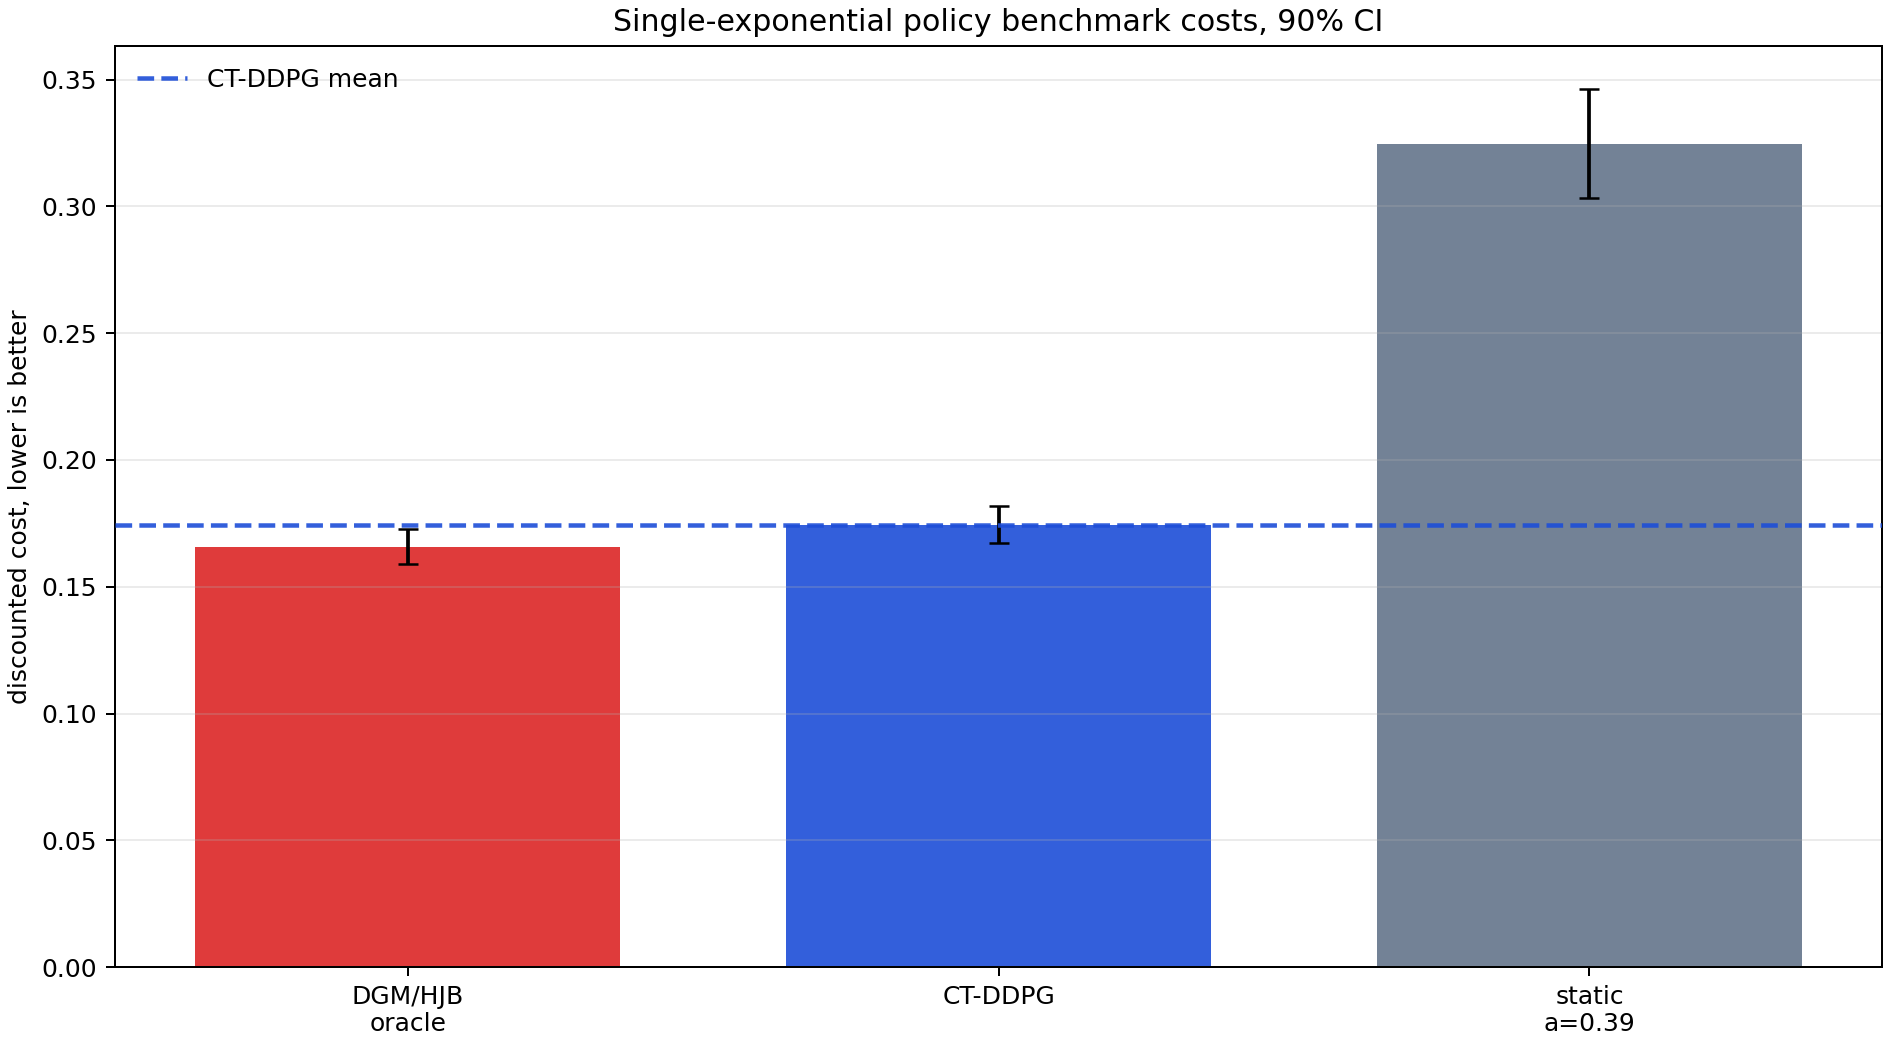
\includegraphics[width=0.96\textwidth]{single_exponential_check_experiment/figures/benchmark_returns.png}
\caption{Single-exponential policy benchmark.}
\label{fig:single-benchmark}
\end{figure}

\begin{figure}[p]
\centering
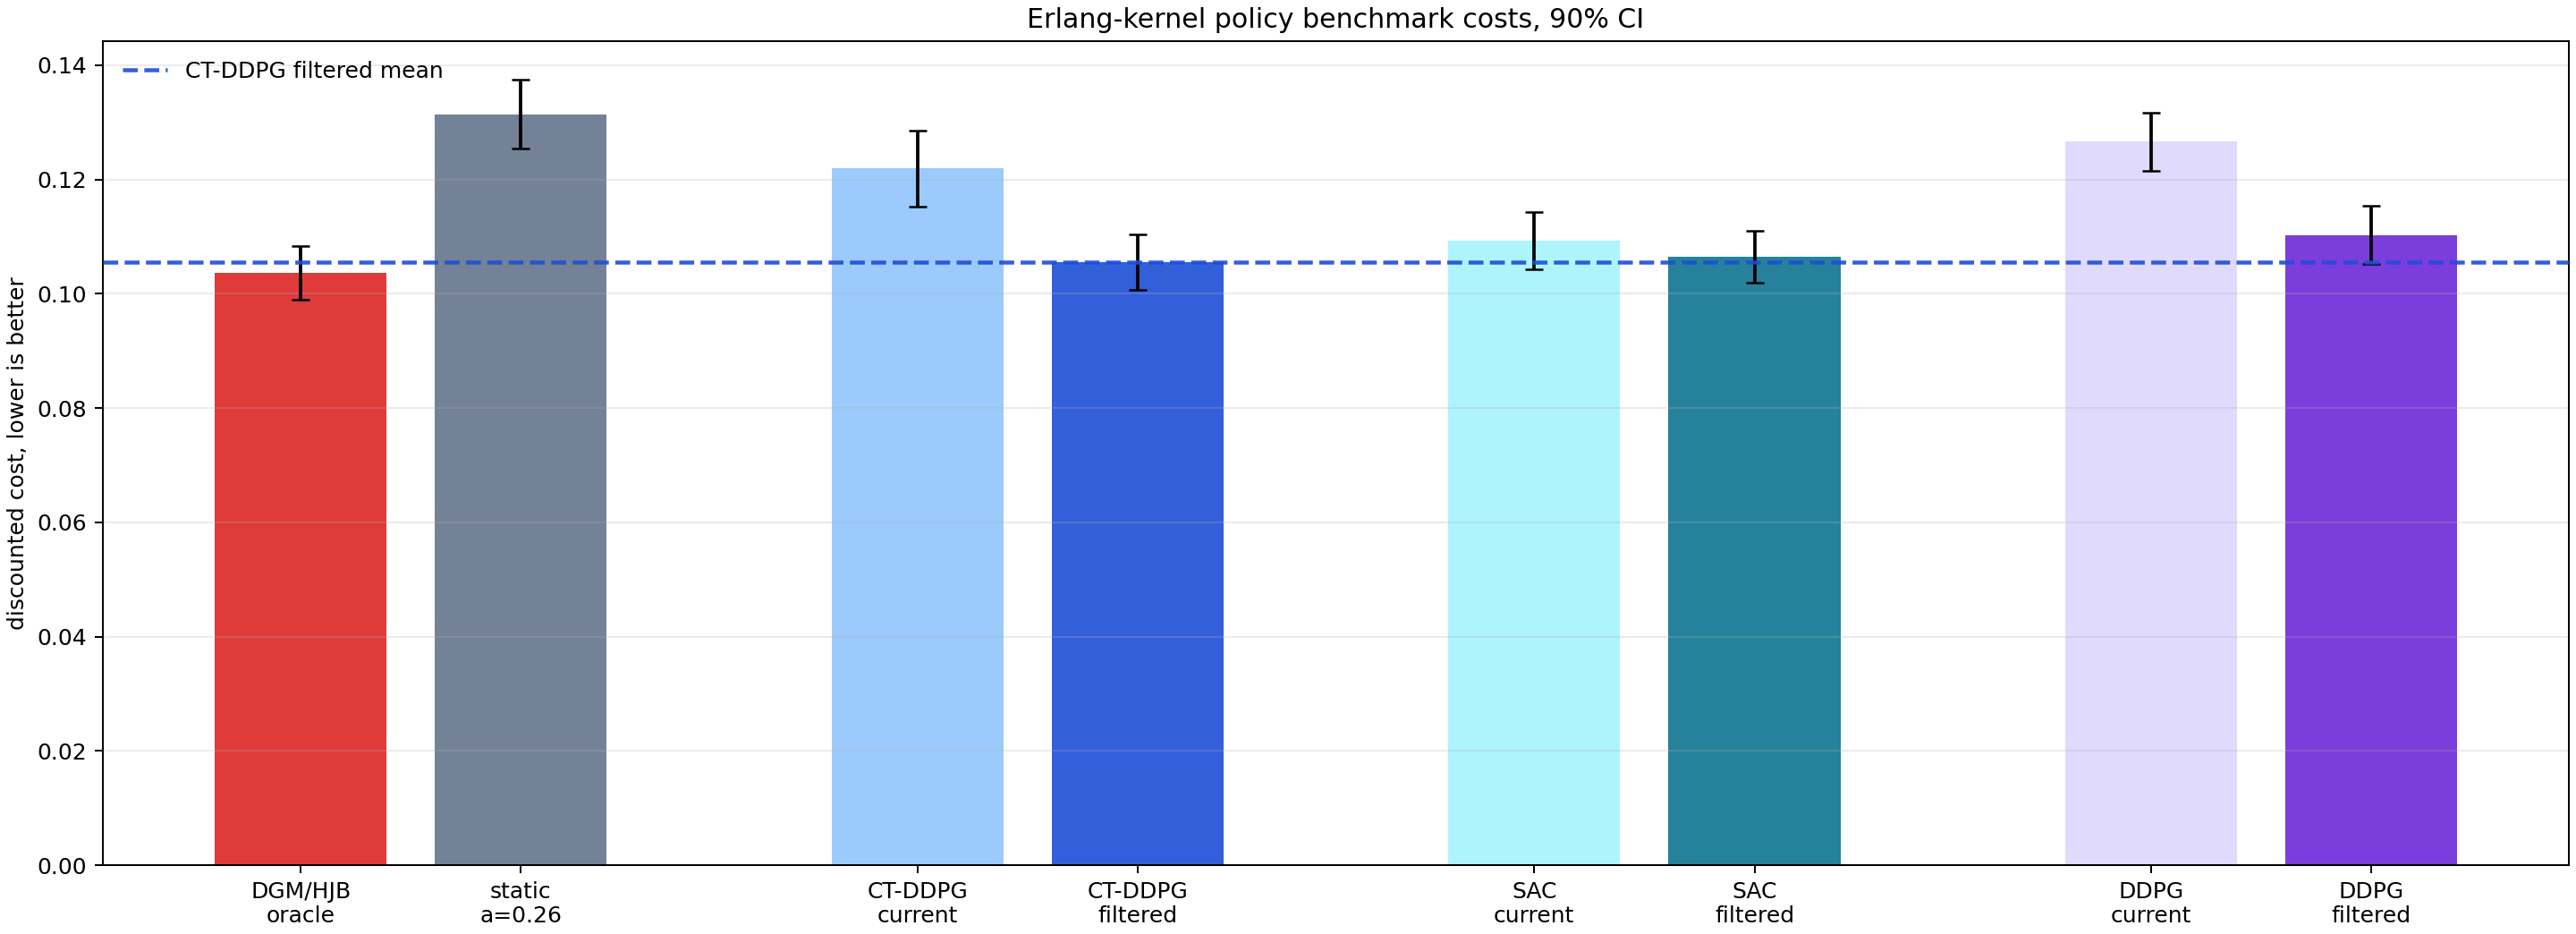
\includegraphics[width=0.96\textwidth]{complex_erlang_experiment/figures/benchmark_returns.png}
\caption{Erlang-kernel policy benchmark under common test paths.}
\label{fig:erlang-benchmark}
\end{figure}

\begin{figure}[p]
\centering
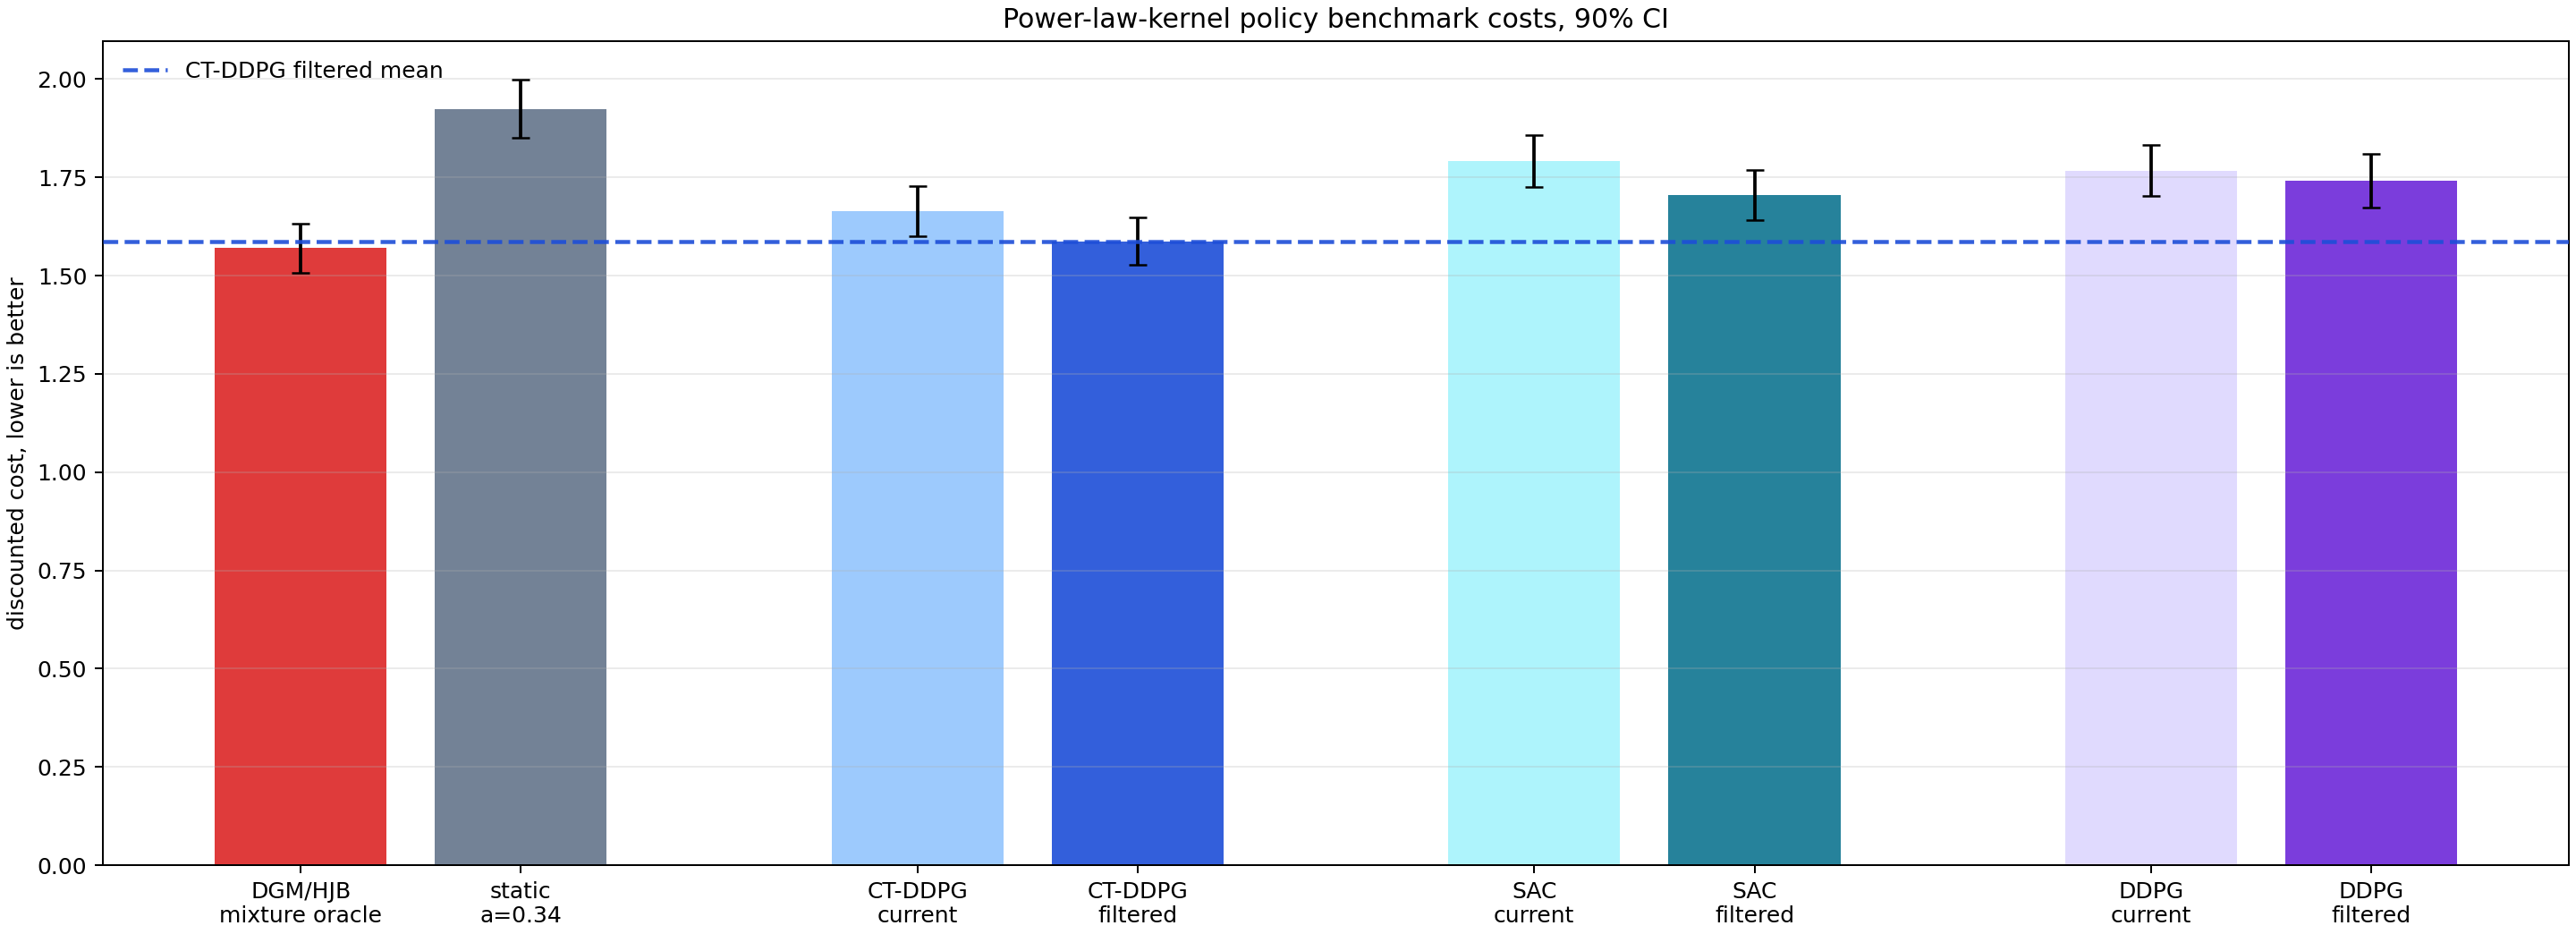
\includegraphics[width=0.96\textwidth]{powerlaw_kernel_experiment/figures/benchmark_costs.png}
\caption{Power-law-kernel policy benchmark under common test paths.}
\label{fig:powerlaw-benchmark}
\end{figure}

\begin{figure}[p]
\centering
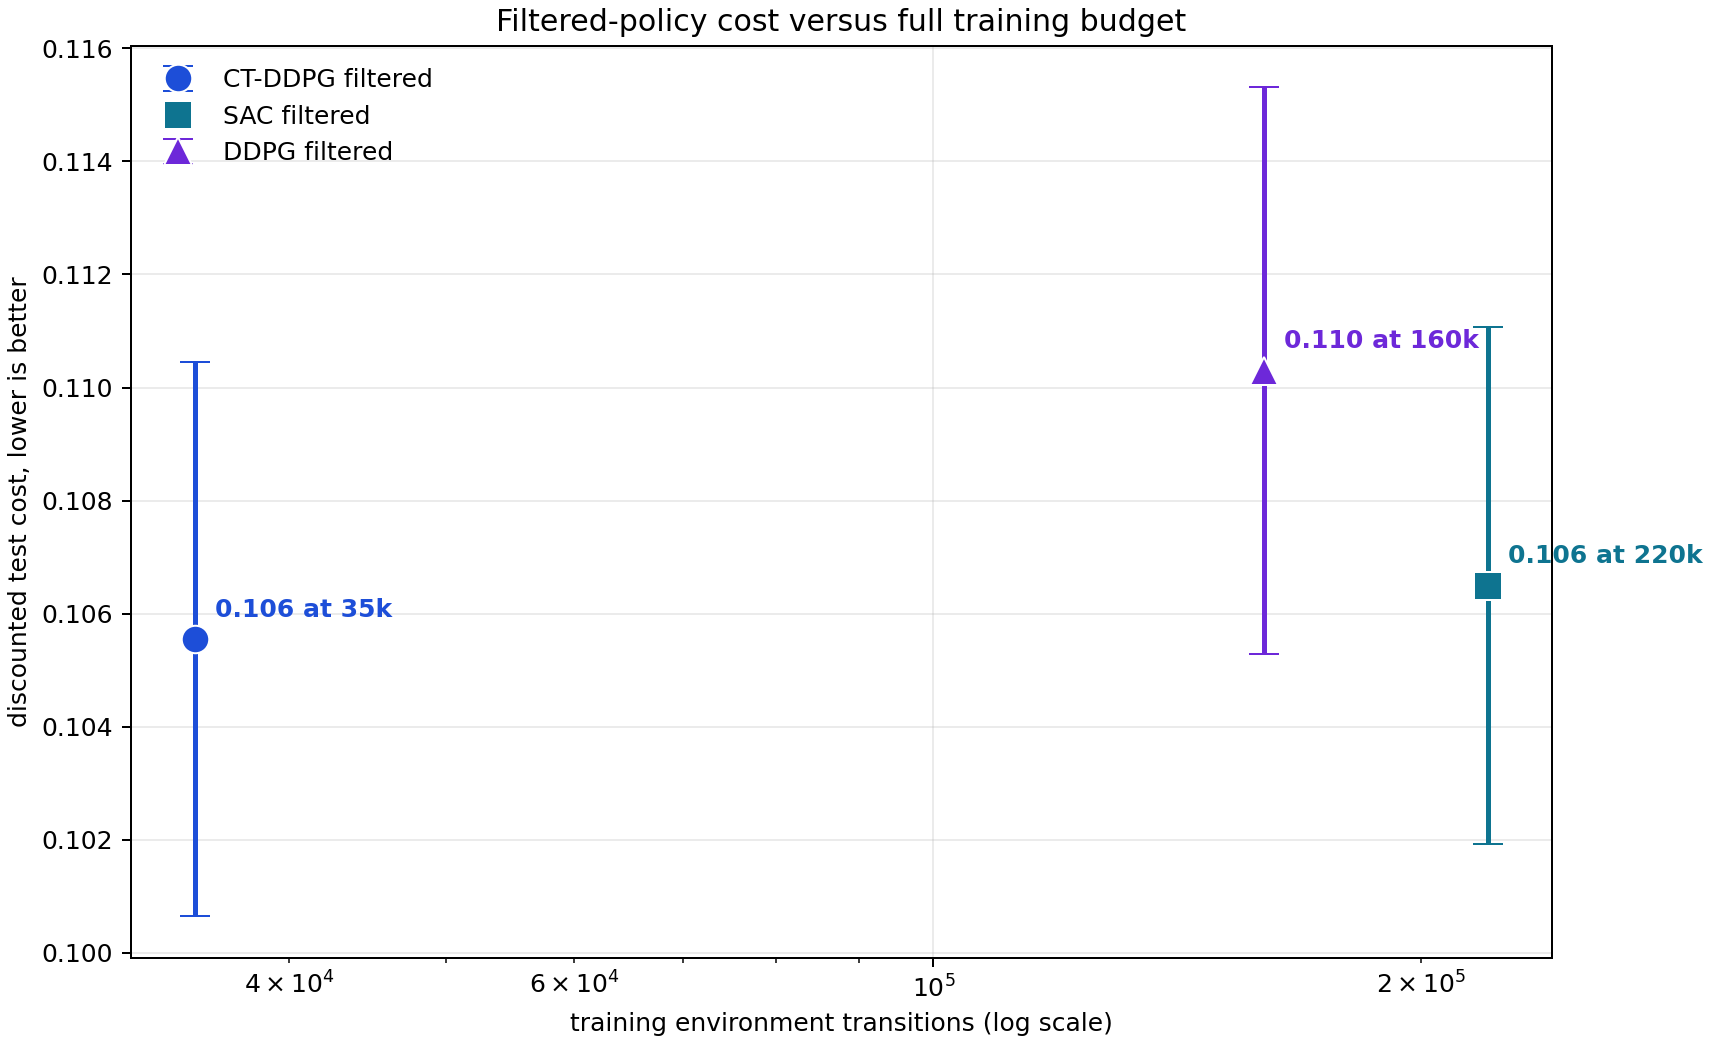
\includegraphics[width=0.96\textwidth]{complex_erlang_experiment/figures/filtered_cost_vs_training_budget.png}
\caption{Erlang filtered-policy cost versus the complete training-transition budget.}
\label{fig:erlang-budget}
\end{figure}

\begin{figure}[p]
\centering
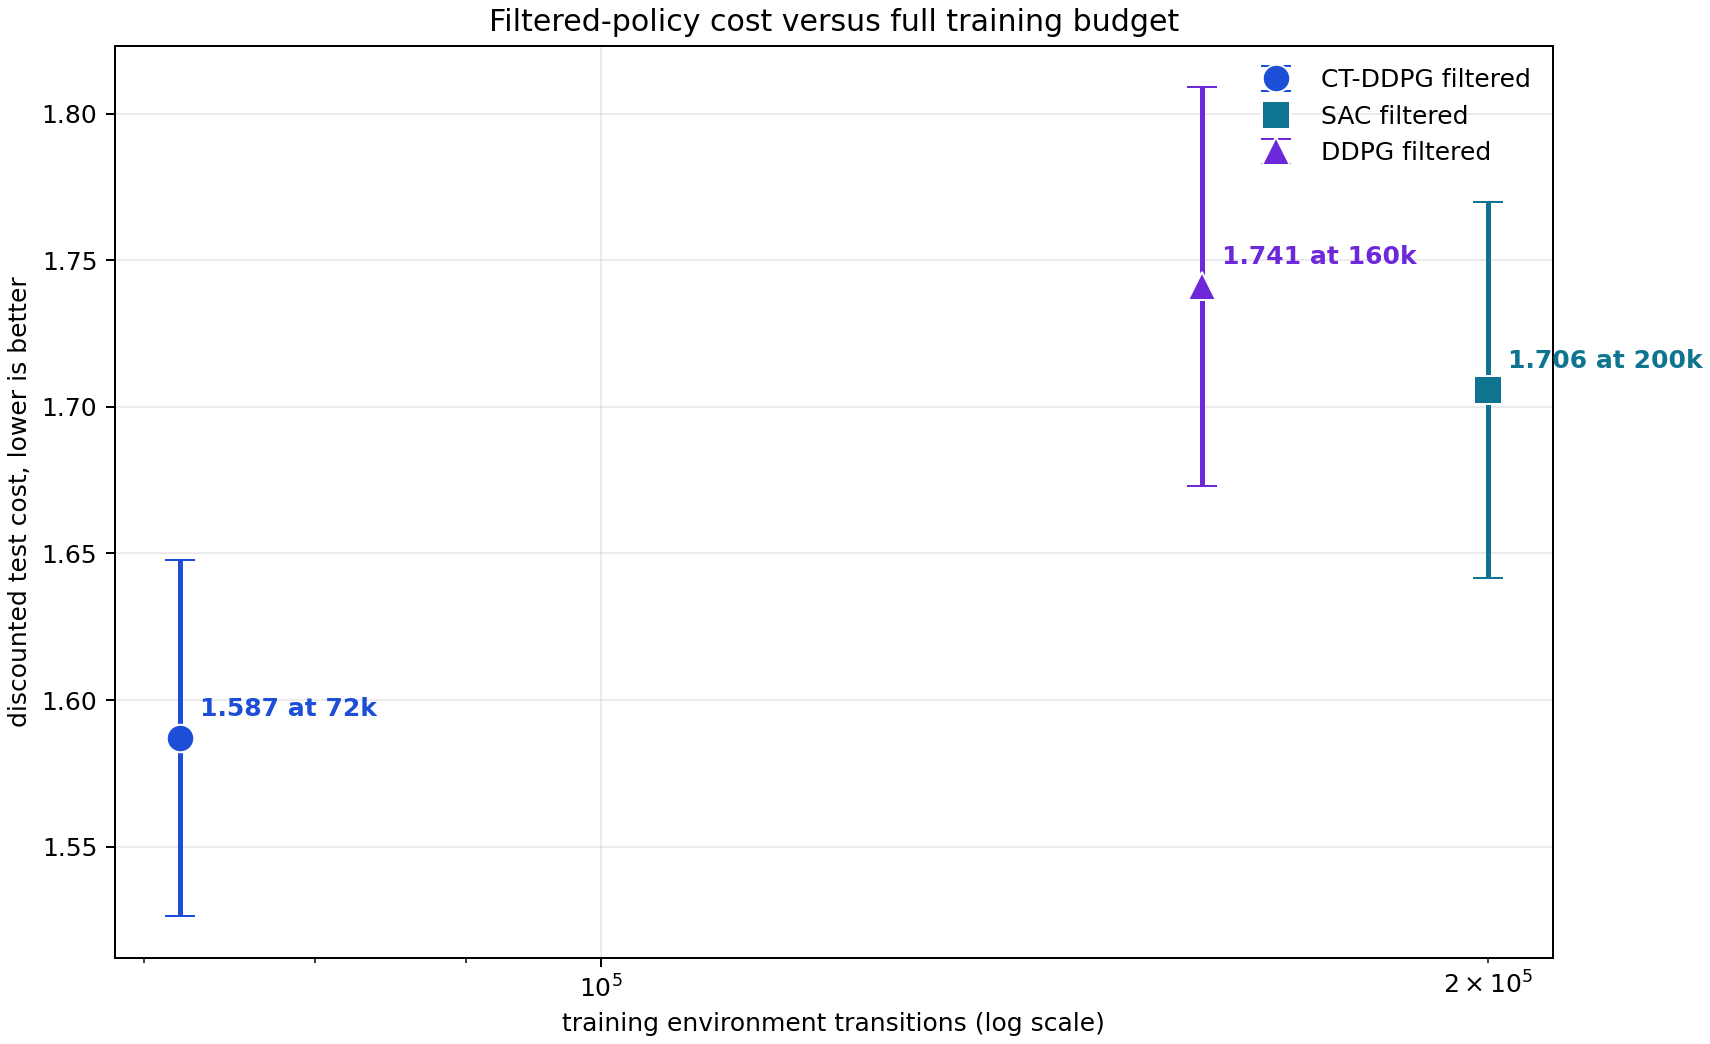
\includegraphics[width=0.96\textwidth]{powerlaw_kernel_experiment/figures/filtered_cost_vs_training_budget.png}
\caption{Power-law filtered-policy cost versus the complete training-transition budget.}
\label{fig:powerlaw-budget}
\end{figure}

\end{document}
